%! Author = Frederik Bußmann
%! Date = 22.06.2023

\section{Umsetzung der CI-Strategie} \label{sec:04-implementation}

Im Folgenden wird die zuvor konzipierte\ \acrshort{ci}-Strategie in die Praxis umgesetzt und dabei in einer Fallstudie
exemplarisch auf ein Projekt angewandt.
Zunächst wird das ausgewählte Projekt vorgestellt, um einen Kontext für die anschließende Implementierung zu schaffen.
Dabei werden die spezifischen Anforderungen und Besonderheiten des Projekts hervorgehoben.
Im Anschluss daran wird die praktische Umsetzung der \acrshort{ci}-Strategie beschrieben, wobei sowohl die technischen
Aspekte als auch die organisatorischen Prozesse berücksichtigt werden.
Hierbei werden\ \acrshort{ci}-Tools für die Strategie ausgewählt, eine Projekt-Struktur und Pipeline definiert und
der eigentliche Shop inklusive angedachter Eigenentwicklungen implementiert.

\subsection{Projekthintergrund} \label{subsec:04-implementation-1}

Bei dem Shopware-Projekt, in welchem die\ \acrshort{ci}-Strategie implementiert werden soll, handelt es sich um einen
Anbieter von Kochutensilien.
Der Shop soll dabei auf der Basis von Shopware 6 neu entwickelt werden und das zuvor erstellte\ \acrshort{ci}-Konzept
in der Praxis einsetzen.
Das Ziel ist hierbei, durch die Integration der untersuchten \acrshort{ci}-Praktiken eine robuste, skalierbare und
effiziente Entwicklungsumgebung zu schaffen, die den Anforderungen moderner Online-Shops gerecht wird.
Dabei wird das zuvor ausgearbeitete \acrshort{ci}-Konzept als Leitfaden für die Entwicklung, Optimierung und
kontinuierliche Qualitätssicherung des Shops herangezogen.
Hierzu wird zunächst eine Shopware-Instanz aufgesetzt, welche anschließend über den Standardumfang der Software hinaus
um ein eigenes Theme und einige Plugins zur Anpassung verschiedener Bereiche des Shops ergänzt wird.
Die für den Shop angedachten Eigenentwicklungen umfassen folgende Plugins:

\begin{itemize}
    \item {
        \textbf{Eigene Produktkacheln auf Listing-Seiten}\par
        Bei Varianten-Artikeln wird keine direkte Auswahlmöglichkeit angeboten, stattdessen werden individuell
        gestaltete Produktkacheln präsentiert.
    }

    \item {
        \textbf{Eigener Produkt-Typ\ \glqq Rezept\grqq}\par
        Dieser spezielle Produkttyp kann vom Kunden betrachtet, aber nicht gekauft werden.
        Er dient zur Präsentation von Rezepten, die mit den im Shop erhältlichen Produkten zubereitet werden können.
    }
\end{itemize}

Als Produkt-Listing-Seiten werden Seiten der Shopware-Instanz bezeichnet, welche die Produkte einer bestimmten
Kategorie oder Gruppierung gesammelt in einer Liste anzeigen.
Produkte werden auf diesen Seiten im Standardumfang der Software als rechteckige Kacheln angezeigt, welche
verschiedene Informationen anzeigen, wie zum Beispiel eine Auswahl an Varianten des Artikels.
Durch das Klicken auf eine der Kacheln wird auf die jeweilige Produkt-Detail-Seite verwiesen.
Diese Seiten zeigen die Detail-Ansicht der Produkte auf und bieten weitere Informationen und Varianten- und
Kaufoptionen.
Für einige weitere benötigte Features des Shops, wie eine Filialsuche und Social-Media-Feeds, wurde der Einsatz von
Drittanbieter-Plugins eingeplant, um Entwicklungszeit einzusparen.

\subsection{Implementierung des Konzepts} \label{subsec:04-implementation-2}

Nachfolgend wird das als Fallstudie vorgesehene Shopware-Projekt anhand der untersuchten\ \acrshort{ci}-Praktiken
implementiert.
Zunächst wird gemäß des Konzepts eine Analyse der zur Verfügung stehenden\ \acrshort{ci}-Tools durchgeführt,
woraufhin Technologien für die Nutzung innerhalb des Projekts ausgewählt werden.
Anschließend wird die Projekt-Umgebung für die Nutzung von\ \acrshort{ci} aufgesetzt und das Shopware-Projekt
installiert und vorbereitet.
Daraufhin wird die Pipeline für das erstellte Projekt angelegt.
Hierbei werden die Phasen und Jobs erstellt und\ \acrshort{ci}-Tools konfiguriert, um automatisierte Tests und Analysen
durchführen zu können.
Nachdem das Projekt initialisiert wurde und die Pipeline funktionsfähig ist, wird die Implementierung der eigentlichen
Shop-Funktionen erläutert, wobei der Fokus auf die kontinuierliche Prüfung der Features durch die Pipeline gerichtet
ist.

\subsubsection{Auswahl von\ \acrshort{ci}-Tools}

Bevor mit der Implementierung des Projekts begonnen werden konnte, musste zunächst analysiert werden, welche Tools
innerhalb des Projekts eingesetzt werden können.
Hierfür wurde eine Analyse verschiedener\ \acrshort{ci}-Tools durchgeführt, wobei eine Auswahl an für das
Projekt zu nutzenden Technologien getroffen wurde:\\

\hspace{0.025\textwidth}%
\begin{minipage}{0.5\textwidth}
    \textbf{Version Control System}
    \vspace{-2mm}
    \begin{itemize}
        \setlength\itemsep{0em}
        \item Git / GitLab
        \item[]
    \end{itemize}
\end{minipage}%
\begin{minipage}{0.475\textwidth}
    \textbf{Pipeline-Runner}
    \vspace{-2mm}
    \begin{itemize}
        \setlength\itemsep{0em}
        \item GitLab CI/CD
        \item[]
    \end{itemize}
\end{minipage}

\hspace{0.025\textwidth}%
\begin{minipage}{0.5\textwidth}
    \textbf{PHP Testing Tools}
    \vspace{-2mm}
    \begin{itemize}
        \setlength\itemsep{0em}
        \item PHPUnit
        \item Infection
        \item[]
    \end{itemize}
\end{minipage}
\begin{minipage}{0.475\textwidth}
    \textbf{JavaScript Testing Tools}
    \vspace{-2mm}
    \begin{itemize}
        \setlength\itemsep{0em}
        \item Jest
        \item Cypress
        \item[]
    \end{itemize}
\end{minipage}

\hspace{0.025\textwidth}%
\begin{minipage}{0.5\textwidth}
    \textbf{PHP Static-Code-Analysis Tools}
    \vspace{-2mm}
    \begin{itemize}
        \setlength\itemsep{0.05em}
        \item PHP\_CodeSniffer
        \item PHP Mess Detector
        \item PHPStan
        \item Deptrac
        \item License Checker
        \item Security Checker
        \item[]
    \end{itemize}
\end{minipage}
\begin{minipage}{0.475\textwidth}
    \textbf{JavaScript Static-Code-Analysis Tools}
    \vspace{-2mm}
    \begin{itemize}
        \setlength\itemsep{-0.05em}
        \item Eslint
        \item Danger JS
        \item License Checker
        \item AuditJS
    \end{itemize}
    \textbf{Deployment Tools}
    \vspace{-2mm}
    \begin{itemize}
        \item Deployer
        \item[]
    \end{itemize}
    \vspace{-4.5mm}
\end{minipage}

Eine vollständige Übersicht und Beschreibung der eingesetzten \acrshort{ci}-Tools kann aus Anhang\ \ref{sec:appendix-1}
entnommen werden.

\subsubsection{Aufsetzen der Projekt-Umgebung}

Nach dem Festlegen der zu verwendenden Technologien wurde mit der Implementierung des Projekts begonnen, wobei
zuerst eine Umgebung für die Ausführung von Shopware und der gewählten\ \acrshort{ci}-Tools erstellt wurde.
Hierbei wurde sich für die Nutzung von Docker als Containerization-Technologie entschieden, da Shopware selbst ein
Docker-Image für das Betreiben der Plattform bereitstellt.\footpartcite{shopware-docker}
Auf der Basis des bereitgestellten Images wurde eine Shopware-Instanz aufgesetzt und anschließend eine Datenbank
angebunden.
Diese wurde, um in der\ \acrshort{ci}-Pipeline wiederverwendet werden zu können, auch aus einem Docker-Image
instanziiert.
Nach der Shopware-Installation wurden Grundkonfigurationen vorgenommen und erste manuelle Tests durchgeführt, um
sicherzustellen, dass die Instanz funktional ist.
\\\\
Nachdem die lokale Entwicklungsumgebung erstellt wurde, konnte mit der Vorbereitung für die Umgebung der Pipelines
begonnen werden.
Hierzu wurde das gesamte Projekt in GitLab hinterlegt und ein Branching-Modell eingeführt, um sicherzustellen, dass
neue Features und Bugfixes vor der Integration in den Hauptzweig (\shellinline{main}) in isolierten Branches entwickelt
werden.
Neben dem\ \shellinline{main}-Branch, welcher als Deployment-Ziel die Produktionsumgebung hinterlegt hat, wurden auch
ein Development-Branch (\shellinline{development}) und -Server angelegt und eine Staging-Umgebung aufgesetzt.
Der Staging-Server ist dabei ein variables Deployment-Ziel, für welches die Auslieferung von
\shellinline{release}-Branches vorgesehen ist.
Die hierbei verwendete Branching-Strategie nennt sich\ \glqq Git-Flow\grqq.
Diese führt Namenskonventionen und verschiedene Arten von Branches ein, wobei neue Features und Anpassungen zunächst in
\shellinline{feature}-Branches entwickelt werden.
Anschließend werden diese in den\ \shellinline{development}-Branch gemerged, wo die Änderungen gesammelt werden.
Die gesammelten Features können daraufhin in einen\ \shellinline{release}-Branch überführt werden, in welchem keine
substantiellen Änderungen sondern nur noch Fehlerbehebungen vorgenommen werden.
\shellinline{release}-Branches können zuletzt in den\ \shellinline{main}-Branch integriert werden.
Dieser stellt den Haupt-Versionsstand des Software-Projekts dar und speichert die aktuell ausgelieferte Version der
Software.
Neben diesen vier Arten von Branches gibt es noch die Möglichkeit,\ \shellinline{hoftix}-Branches für Fehlerbehebungen,
welche am Haupt-Versionsstand vorgenommen werden müssen.\footpartcite{git-flow}

\subsubsection{Erstellen der Pipeline}

Nachdem eine ausführende Umgebung definiert wurde, kann nun die eigentliche Pipeline für das Projekt erstellt werden.
Diese soll zunächst bei jeder Integration in einen Branch ausgeführt werden und durchläuft dabei eine Build-,
Testing- und Deployment-Stage.
Im Build-Prozess werden die \acrshort{ci}-Tools und die Abhängigkeiten der Shopware-Platform installiert.
Der Testing-Prozess umfasst zunächst alle für die Strategie ausgewählten Testing- und \acrshort{qa}-Tools, inklusive
lang-andauernder Tests durch End-to-End-Testing.
Im späteren Verlauf der Entwicklung besteht durch Gitlab CI/CD die Möglichkeit, diese Tests nur in Branches mit
definierter Deployment-Umgebung durchführen zu lassen, falls dessen Laufzeit zu groß wird.
Abschließend liefern Jobs in der Deployment-Stage den entwickelten Code an die jeweilig für den Branch definierte
Umgebung aus.
\\\\
In Abbildung\ \ref{fig:ci-pipeline-concept} wird die für das Projekt erstellte\ \acrshort{ci}-Pipeline vorgestellt.
Hierbei werden verschiedene Arten von Branches in einem\ \acrshort{vcs} dargestellt, welche zunächst die gleiche Aktion
auslösen, den Build-Prozess.
Dort werden die \acrshort{ci}-Tools und die Abhängigkeiten von Shopware für die anschließende Nutzung in der
Testing-Stage installiert.
Die Testing-Stage wird nach erfolgreichem Durchlaufen der Build-Stage ausgeführt und ist in der Abbildung in zwei
Teile separiert.
Im oberen Teil werden die gewählten Testing- und \acrshort{qa}-Tools für JavaScript-Code der Strategie aufgezeigt,
während der untere Teil die Tools für PHP darstellt.
Wenn alle Jobs der Testing-Stage erfolgreich durchgelaufen sind, wird, je nach Art des Ausgangs-Branches, ein
Deployment-Prozess für die jeweilige Umgebung angestoßen.
Die Deployment-Stage wird nur für Branches mit definierter Umgebung ausgeführt und liefert dabei den Code des
Ausgangs-Branches an den Development-, Staging- oder Produktions-Server aus.

\begin{figure}[H]
    \centering
    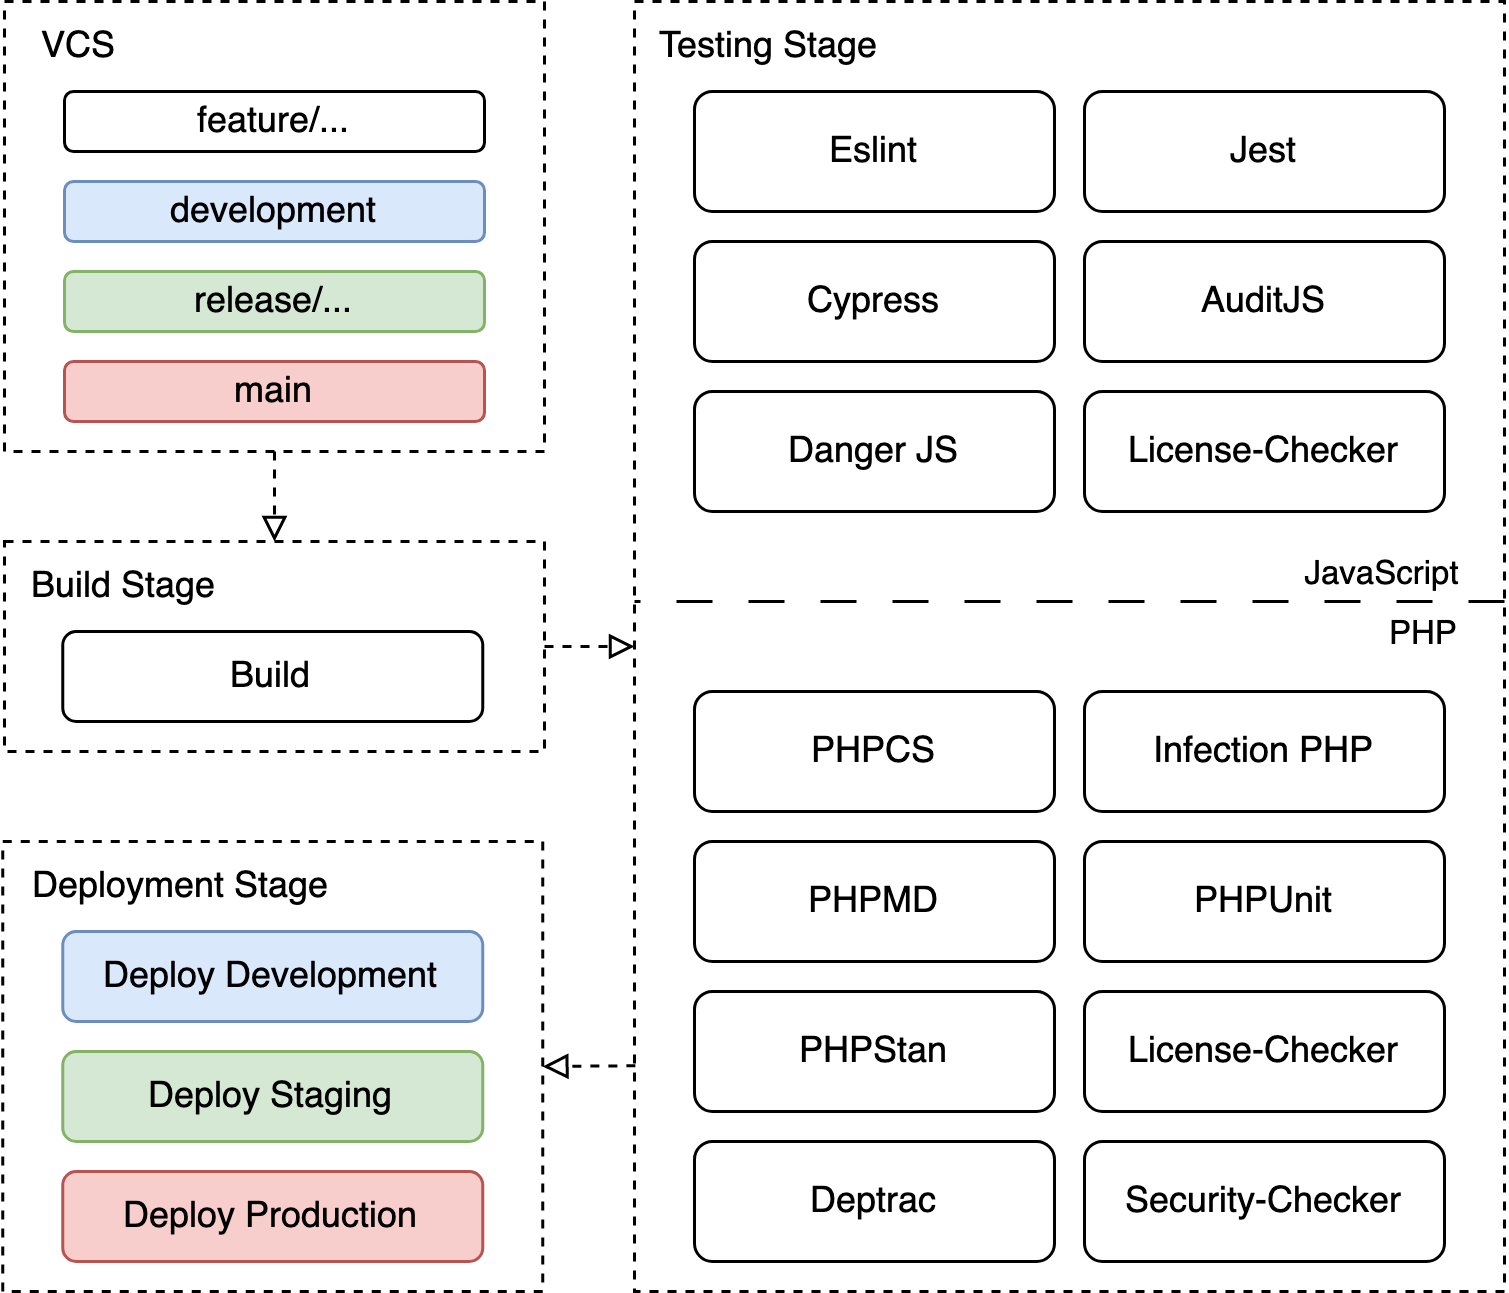
\includegraphics[width=0.69420\textwidth]{images/content/ci-pipeline-concept}
    \captioncite[Eigene Darstellung]{}{Visualisierung der implementierten\ \acrshort{ci}-Pipeline}
    \label{fig:ci-pipeline-concept}
\end{figure}

Die visuelle Ausgabe durchgeführter Pipelines des Projekts durch GitLab CI/CD kann aus Anhang\ \ref{sec:appendix-2}
entnommen werden.

\subsubsection{Implementierung der Shop-Funktionen}

Durch die zuvor erstellten Umgebungen und die angelegte Pipeline-Konfiguration konnten nun die geplanten Funktionen des
Shops unter der Nutzung der erarbeiteten\ \acrshort{ci}-Praktiken implementiert werden.
Diese können grob in drei verschiedene Bereiche eingeteilt werden:

\begin{itemize}
    \item {
        \textbf{Entwicklung des Shop-Themes}\par
        Bei der Entwicklung des Themes für die Shopware-Instanz handelt es sich um viele kleine Anpassungen an dem
        bestehenden User Interface (\acrshort{ui}) des Standardumfangs.
        Da\ \acrshort{ui}-Anpassungen aufwändig zu testen sind und die Standard-\acrshort{ui} durch
        Shopwares eigene Tests abgedeckt ist, wurde das Theme ohne weitere Tests angelegt.
        Für Anpassungen, welche substantiell die Funktion von\ \acrshort{ui}-Komponenten verändern, können jedoch
        System-Tests angelegt werden, wobei geprüft wird, ob sich die angepasste\ \acrshort{ui} nach den gegebenen
        Vorschriften verhält.
        Dies hat den Vorteil dass Bugs, die durch Updates der Standard-\acrshort{ui} mit bestehenden Anpassungen
        entstehen, schneller erkannt und gefixed werden können.
    }

    \item {
        \textbf{Entwicklung des Plugins zur Anpassung der Produktkacheln}\par
        Um die angepassten Produktkacheln zu entwickeln, wurde ein eigenes Plugin angedacht, welches bestimmte
        Produkt-Daten in den Kacheln auf Produkt-Listing-Seiten des Shops anzeigt.
        Hier wird im Standard-Umfang der Shopware-Platform eine Auswahl an Varianten angeboten, welche durch das
        Plugin ersetzt werden soll.
        Statt der Variantenauswahl, soll an dieser Stelle der Preis der günstigsten Variante angezeigt werden.
        Bei der Integration dieses Plugins konnten verschiedene Bereiche durch den Einsatz der Pipeline auf ihre
        Richtigkeit geprüft werden.
        Da die günstigste Artikelvariante zunächst Backend-Seitig bestimmt und dem Frontend zur Verfügung
        gestellt werden musste, wurde bei der Entwicklung PHP-Code produziert.
        Für diesen konnten Unit-, Module- und Integration-Tests angelegt und dazugehörige\ \acrshort{ui}-Anpassungen
        im Frontend durch System-Tests abgedeckt werden.
        Die generelle Einhaltung gesetzter Code-Standards und weitere Qualitätsmerkmale wurden hierbei durch die
        gewählten statischen Code-Analyse-Tools überwacht.
    }

    \item {
        \textbf{Entwicklung des Plugins für Rezept-Produkte}\par
        Das Plugin für die Erstellung von Rezepten legt eine eigene Produkt-Art an, welche nicht aktiv im Shop gekauft
        werden kann und dabei lediglich die hinterlegten Rezept-Informationen anzeigt.
        Da dieses Feature sowohl Backend- als auch Frontend-Anpassungen benötigt, konnte der entwickelte PHP- und
        JavaScript-Code ebenfalls durch Unit-, Module- und Integration-Tests abdeckt werden.
        Die frontend-seitigen Erweiterungen bestimmter Produkt-Kacheln im Listing und der Produkt-Detail-Seite, welche
        nun Rezepte statt Produkten anzeigen, wurden dabei auch durch System-Tests abgedeckt.
        Vorteilhaft bei dieser Art der automatisierten Prüfung der erstellten Features ist, dass mit neuen
        Entwicklungen eingeführte Wechselwirkungen und Fehler schneller entdeckt werden können.
        So wurde zum Beispiel durch Regression- und System-Tests verhindert, dass das Anpassen der Produktkacheln
        durch beide erstellten Plugins zu unentdeckten Problemen nach der Integrationsphase führt.
    }
\end{itemize}

Bei der Entwicklung der Anpassungen wurden verschiedene\ \acrshort{ci}-Praktiken und Tools eingesetzt.
Der für die Anpassungen entwickelte PHP- und JavaScript-Code konnte hierbei durch automatisierte Unit-, Module- und
Integration-Tests der Tools\ \shellinline{PHPUnit} und\ \shellinline{Jest} abgedeckt werden.
Erstellte Unit-Tests in PHP wurden durch das \shellinline{Infection}-Framework mit Mutation-Tests kontinuierlich
evaluiert.
System-Tests konnten mit dem JavaScript-basierten Tool\ \shellinline{Cypress} erstellt und durchgeführt werden.
Durch\ \shellinline{Deptrac} konnte die Architektur der erstellten PHP-Klassen und Module geprüft werden.
Die Einhaltung gesetzter Coding-Standards und weitere Qualitätsmetriken konnten durch die Nutzung von
\shellinline{PHPCS}, \shellinline{PHPMD} und \shellinline{PHPStan} für PHP-Code und von \shellinline{Eslint} für
JavaScript-Code erhoben werden.
\shellinline{AuditJS} und der PHP\ \shellinline{Security Checker} konnten installierte Pakete automatisch auf
Sicherheitslücken überprüfen.
Um die Lizenzen der im Projekt installierten Pakete für das Projekt zu überwachen, wurden\ \shellinline{License Checker}
eingesetzt, welche die Lizenzen der von Composer und\ \acrshort{npm} installierten Pakete beobachten.
Außerdem wurde\ \shellinline{Danger JS} zur steigerung der Transparenz des\ \acrshort{ci}-Prozesses eingesetzt, welches
den Status der einzelnen Jobs einer durchgelaufenen Pipeline in Form eines Kommentars im\ \acrshort{vcs} hinterlegt.
Letztlich wurden die Deployments für die jeweiligen Umgebungen durch das PHP-basierte Tool\ \shellinline{Deployer}
durchgeführt, wodurch die Ausfallzeiten beim Ausliefern der Software minimiert werden konnten.
\\\\
Drittanbieter-Plugins und Shop-Konfigurationen wurden hierbei nicht weiter getestet, da es sich nicht um
Eigenentwicklungen handelt und diese durch die jeweiligen Hersteller oder die Shopware-Platform selbst geprüft werden.
Außerdem wurden im Verlauf des Projekts neben den automatisierten Tests durch die\ \acrshort{ci}-Pipeline auch
manuelle Tests von Entwicklern, Projektleitern und den Kunden durchgeführt, um die System-Funktionalität
sicherzustellen.
Darüber hinaus wurde durch die Verwendung einer flexiblen Pipeline die Möglichkeit eingeräumt, das Projekt durch
Performance- und Last-Tests zu überwachen oder weitere Tools und Services zum Testen der Applikation anzubinden.
Dank des parallelen Ausführens der Test-Jobs konnte die Durchlaufzeit der Pipeline minimiert werden, wobei die
Strategie auch die Möglichkeit bietet Jobs konditionell auszuführen, sollte deren Dauer die gesetzte Zehn-Minuten-Marke
übersteigen.

\clearpage
